\section{Conceptual Modelling}\label{sec:cm}

Data modeling is the practice of using words and symbols to represent data and how it flows in a simplified representation of a software system and the data pieces it includes. Data models serve as a road-map for creating a new database or re-engineering an existing one. A data model is a flowchart that depicts data items, their properties, and the relationships that exist between them. Before any code is developed, it allows data management and analytic teams to establish data needs for apps and uncover mistakes in development plans.\\
Data models can generally be divided into three categories, which vary according to their degree of abstraction. The process will start with a conceptual model, progress to a logical model and conclude with a physical model. We describe conceptual data modeling in this section.\\

In software development, conceptual data modeling is a concept that represents the relationships between different entities in a database. This data model is generated as a result of the requirement analysis and is the most basic type of data modeling. Therefore, this paradigm, which is known as extremely abstract, is easy to understand by any technician or non-technical person. In this data model, the entity's attributes may or may not be present. Business stakeholders and data architects are frequently involved in the creation of this data model. 
We analyzed our project requirements and developed a very basic data model (Conceptual Data Model), which is shown below.

\begin{figure}[H]
    \centering
    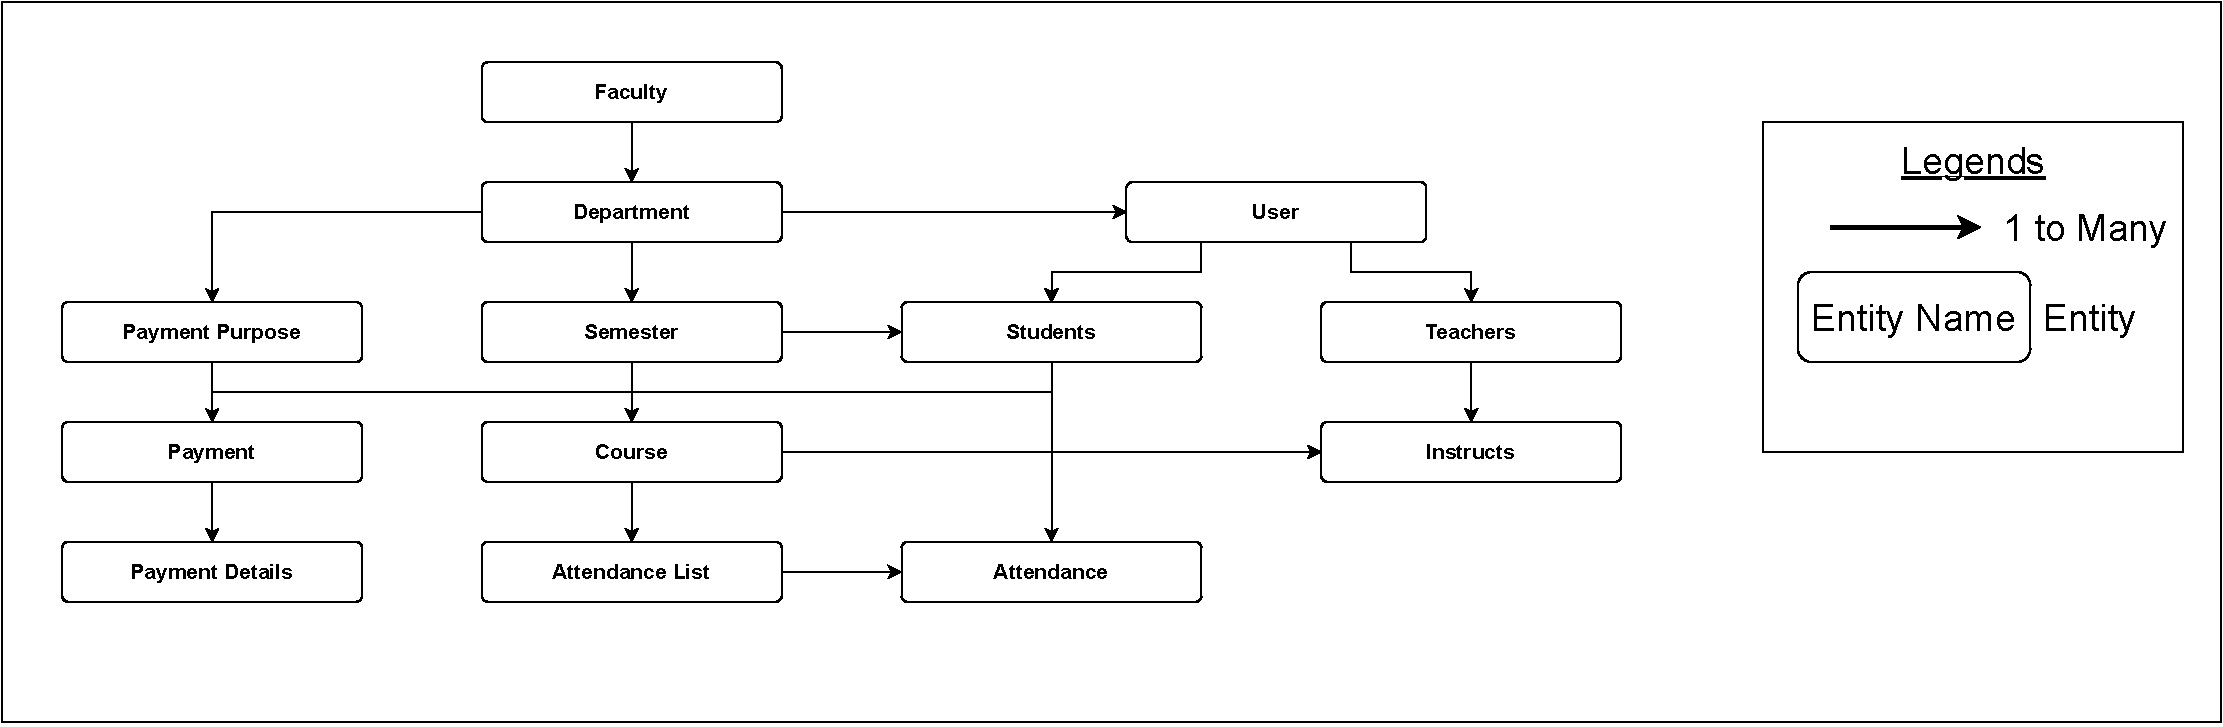
\includegraphics[width=1\textwidth]{images/conceptual}
    \caption{Conceptual Data Model of CU-OPAS}
    \label{fig:conceptual}
\end{figure}